\documentclass{article}
\usepackage[utf8]{inputenc}
\usepackage{amsmath}
\usepackage{amssymb}
\usepackage{graphicx}
\usepackage{xcolor}


\begin{document}

\section*{Structured linear systems}
In this exercise we consider the linear system $\mathbf{A}\mathbf{x} = \mathbf{b}$ where the $n \times n$ matrix $\mathbf{A}$ has the following structure 
\begin{equation*}
    \mathbf{A} = \begin{bmatrix}
    a_{1}& 0 & 0 & \dots & 0 \\
    a_{1} & a_{2}& 0 & \ddots & \vdots \\
    a_{1} & a_{2} & a_{3} & \ddots & \\
    \vdots & \vdots & \vdots& \ddots & 0 \\
    a_{1} & a_{2} & a_{3} & \dots & a_{n}
    \end{bmatrix}
\end{equation*}
\subsection*{2-12.a} 
We are tasked with giving a sufficient condition for the vector $\mathbf{a} = \left(a_{1}, \dots, a_{n}\right)^{\mathsf{T}} \in \mathbb{R}^{n}$ such that the matrix $\mathbf{A}$ is non-singular. We have
\begin{equation*}
    \mathbf{A} \text{ is non-singular } \Longleftrightarrow \mathbf{A} \text{ is regular } \Longleftrightarrow \text{det}\left(\mathbf{A}\right) \neq 0
\end{equation*}
and the determinant of a triangular matrix is the product of its diagonal element, i.e.
\begin{equation*}
    \text{det}\left(\mathbf{A}\right) = a_{1} \cdot \: \dots \: \cdot a_{n}
\end{equation*}
hence for $\text{det}\left(\mathbf{A}\right) \neq 0$ to be the case we must have that none of the diagonal elements are zero
\begin{equation*}
    \mathbf{A} \text{ is non-singular } \Longleftrightarrow a_{i} \neq 0 \quad \forall \, i \in \left\{1, \dots, n\right\}
\end{equation*}
\subsection*{2-12.b}
We are tasked with writing a function that builds a matrix $\mathbf{A}$ according to the above structure given the vector $\mathbf{a} = \left(a_{1}, \dots, a_{n}\right)^{\mathsf{T}}$. We can make use of \verb|head(amount)| here which allows us to access the \verb|amount| first elements of a vector. In our case we will set each row separately or we can use a nested for loop. Both options are valid and we will implement both. Let us first look at how \verb|head| and \verb|tail| work
\begin{equation*}
\mathbf{A} = 
    \begin{bmatrix}
        a_{1} & 0 & 0 & 0 & 0 & 0 \\
        a_{1} & a_{2} & 0 & 0 & 0 & 0 \\
        \color{red}a_{1}\color{black} & \color{red}a_{2}\color{black} & \color{red}a_{3}\color{black} & 0 & 0 & 0 \\
        a_{1} & a_{2} & a_{3} & \color{blue}a_{4}\color{black} & 0 & 0 \\
        a_{1} & a_{2} & a_{3} & \color{blue}a_{4}\color{black} & a_{5} & 0 \\
        a_{1} & a_{2} & a_{3} & \color{blue}a_{4}\color{black} & a_{5} & a_{6} \\
    \end{bmatrix} 
\end{equation*}
We have (we use \verb|C++| indexing) that the red segment is given by \color{red}\verb|A.row(2).head(3)|\color{black} and the blue segment is given by \color{blue}\verb|A.col(3).tail(3)|\color{black}. This is how we will access and assign the rows and columns of the matrix (we will use \verb|head|) in our implementation.

\pagebreak

\noindent The for loop based approach is pretty straight forward
\begin{figure}[!hbt]
    \centering
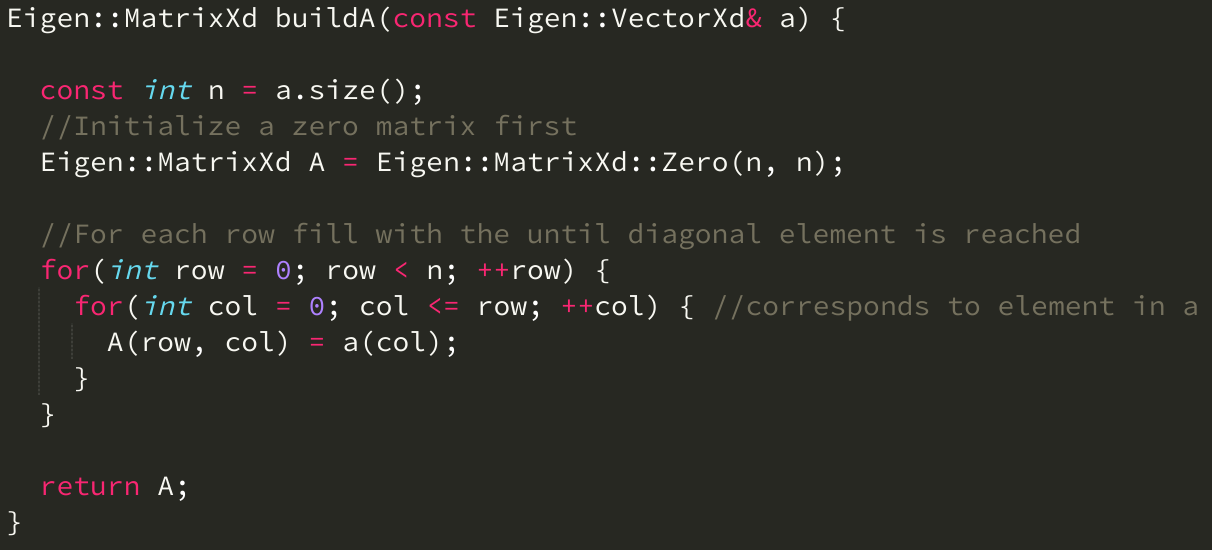
\includegraphics[width=1.0\linewidth]{2-12.b1.png}
\end{figure}

\noindent The \verb|head| access based approach looks more complicated but works very similar

\begin{figure}[!hbt]
    \centering
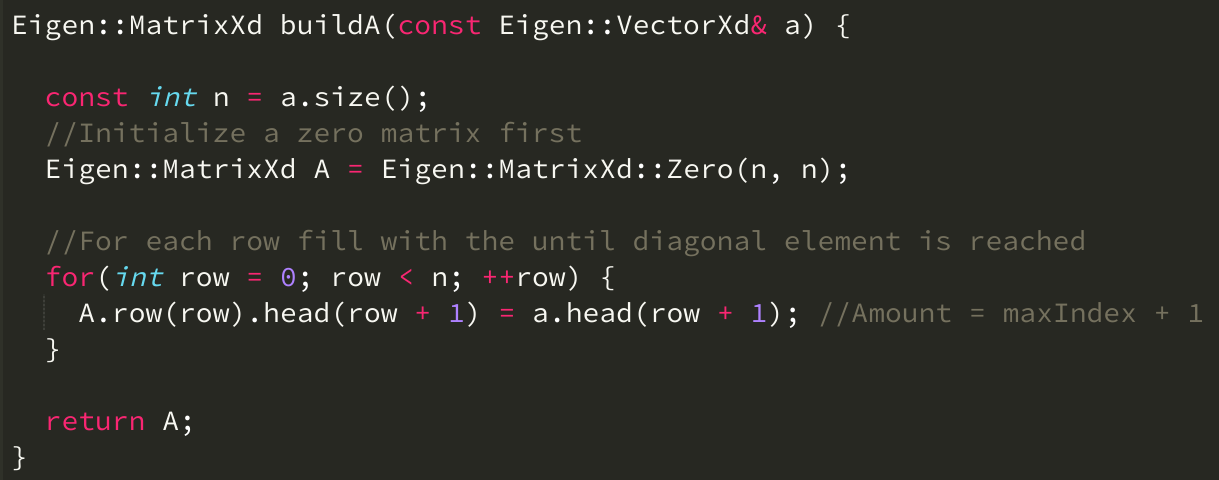
\includegraphics[width=1.0\linewidth]{2-12.b2.png}
\end{figure}
\subsection*{2-12.c}
We are now tasked with implementing a \verb|C++| function that solves the linear system $\mathbf{A}\mathbf{x} = \mathbf{b}$ and \textbf{not} using the structure of $\mathbf{A}$. We use \verb|Eigen::PartialPivLU| to give us the LU decomposition of $\mathbf{A}$ which we can construct using one of the methods above. This we can do in the following way \\[2mm]
\verb|x = LU.solve(b)|
\\[1mm]
this solves the system $\mathbf{A}\mathbf{x} = \mathbf{b}$.

\pagebreak

\noindent This produces the following code
\begin{figure}[!hbt]
    \centering
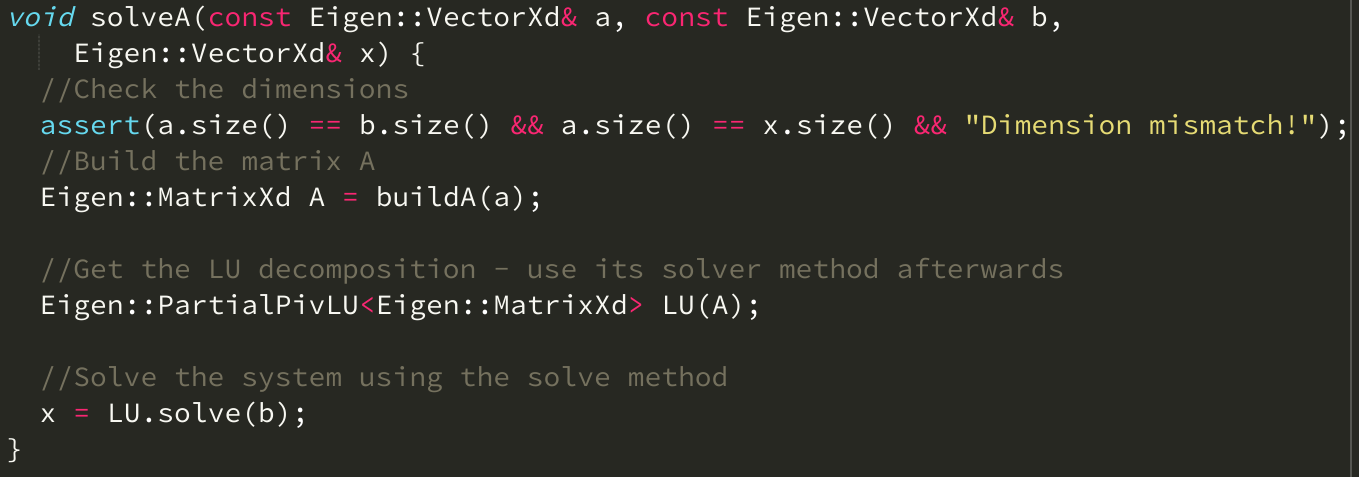
\includegraphics[width=1.0\linewidth]{2-12.c.png}
\end{figure}
The asymptotic complexity can be determined by looking at what methods we use. The assertion is takes $\mathcal{O}\left(1\right)$, the construction of $\mathbf{A}$ is in $\mathcal{O}\left(n^{2}\right)$, the LU-decomposition takes $\mathcal{O}\left(n^{3}\right)$ to be computed and the system can then be solved in $\mathcal{O}\left(n^{2}\right)$, resulting in $\mathcal{O}\left(n^{3}\right)$ overall.
\subsection*{2-12.d}
We are now tasked for a generic $\mathbf{a} \in \mathbb{R}^{n}$ to compute by hand the inverse of the matrix $\mathbf{A}$ and then from this the solution $\mathbf{x}$ of $\mathbf{A}\mathbf{x} = \mathbf{b}$. The hint tells us the following equality
\begin{equation*}
\mathbf{A} =
    \begin{bmatrix}
        a_{1}& 0 & 0 & \dots & 0 \\
    a_{1} & a_{2}& 0 & \ddots & \vdots \\
    a_{1} & a_{2} & a_{3} & \ddots & \\
    \vdots & \vdots & \vdots& \ddots & 0 \\
    a_{1} & a_{2} & a_{3} & \dots & a_{n}
    \end{bmatrix} =  \begin{bmatrix}
        1& 0 & 0 & \dots & 0 \\
    1 & 1& 0 & \ddots & \vdots \\
    1 & 1 & 1 & \ddots & \\
    \vdots & \vdots & \vdots& \ddots & 0 \\
    1 & 1& 1 & \dots & 1
    \end{bmatrix} \begin{bmatrix}
        a_{1}& 0 & 0 & \dots & 0 \\
    0 & a_{2}& 0 & \ddots & \vdots \\
    0& 0 & a_{3} & \ddots & \\
    \vdots & \vdots & \vdots& \ddots & 0 \\
    0 & 0 & 0 & \dots & a_{n}
    \end{bmatrix} = \mathbf{E} \cdot \mathbf{D}
\end{equation*}
Both these matrices are invertible if $\mathbf{A}$ is invertible because $\mathbf{A}$ being invertible means it is regular and thus as discussed above $a_{i} \neq 0$ for all $1\leq i \leq n$. Hence the product of the diagonal of both the lower triangular matrix $\mathbf{E}$ and the diagonal matrix $\mathbf{D}$ are non-zero and thus both matrices are regular (In general if the product of two matrices is regular then they are both regular, so this would not be needed to state here.). We can then use that
\begin{equation*}
    \mathbf{A}^{-1} = \left(\mathbf{E}\cdot \mathbf{D}\right)^{-1} = \mathbf{D}^{-1}\cdot \mathbf{E}^{-1}
\end{equation*}
The inverse of the diagonal matrix is given by
\begin{equation*}
    \mathbf{D}^{-1} = \begin{bmatrix}
        \frac{1}{a_{1}}& 0 & 0 & \dots & 0 \\
    0 & \frac{1}{a_{2}}& 0 & \ddots & \vdots \\
    0& 0 & \frac{1}{a_{3}} & \ddots & \\
    \vdots & \vdots & \vdots& \ddots & 0 \\
    0 & 0 & 0 & \dots & \frac{1}{a_{n}}
    \end{bmatrix}
\end{equation*}


\noindent Let us look at the inverse of $\mathbf{E}$. We use the algorithm learned in the linear algebra lecture to do find the inverse of a small example
\begin{align*}
    \begin{array}{cccc|cccc}
    \mathbf{1} & \mathbf{0} & \mathbf{0} & \mathbf{0} & \mathbf{1} & \mathbf{0} & \mathbf{0} & \mathbf{0} \\
    1 & 1 & 0 & 0 & 0 & 1 & 0 & 0 \\
    1 & 1 & 1 & 0 & 0 & 0 & 1 & 0 \\
    1 & 1 & 1 & 1 & 0 & 0 & 0 & 1 
    \end{array} &\longrightarrow \begin{array}{cccc|cccc}
    1 & 0 & 0 & 0 & 1 & 0 & 0 & 0 \\
    0 & 1 & 0 & 0 & -1 & 1 & 0 & 0 \\
    0 & 1 & 1 & 0 & -1& 0 & 1 & 0 \\
    0 & 1 & 1 & 1 & -1 & 0 & 0 & 1 
    \end{array} \\
    \begin{array}{cccc|cccc}
    1 & 0 & 0 & 0 & 1 & 0 & 0 & 0 \\
    \mathbf{0} & \mathbf{1} & \mathbf{0} & \mathbf{0} & \mathbf{-1} & \mathbf{1} & \mathbf{0} & \mathbf{0} \\
    0 & 1 & 1 & 0 & -1& 0 & 1 & 0 \\
    0 & 1 & 1 & 1 & -1 & 0 & 0 & 1 
    \end{array} &\longrightarrow
    \begin{array}{cccc|cccc}
    1 & 0 & 0 & 0 & 1 & 0 & 0 & 0 \\
    0 & 1 & 0 & 0 & -1 & 1 & 0 & 0 \\
    0 & 0 & 1 & 0 & 0& -1 & 1 & 0 \\
    0 & 0 & 1 & 1 & 0 & -1 & 0 & 1 
    \end{array} \\
    \begin{array}{cccc|cccc}
    1 & 0 & 0 & 0 & 1 & 0 & 0 & 0 \\
    0 & 1 & 0 & 0 & -1 & 1 & 0 & 0 \\
    \mathbf{0} & \mathbf{0} & \mathbf{1} & \mathbf{0} & \mathbf{0}& \mathbf{-1} & \mathbf{1} & \mathbf{0} \\
    0 & 0 & 1 & 1 & 0 & -1 & 0 & 1 
    \end{array} &\longrightarrow
    \begin{array}{cccc|cccc}
    1 & 0 & 0 & 0 & 1 & 0 & 0 & 0 \\
    0 & 1 & 0 & 0 & -1 & 1 & 0 & 0 \\
    0 & 0 & 1 & 0 & 0& -1 & 1 & 0 \\
    0 & 0 & 0 & 1 & 0 & 0 & -1 & 1 
    \end{array}
\end{align*}
We now have the identity matrix on the left and the inverse on the right, the pattern we found here can be generalized and we get 
\begin{equation*}
    \mathbf{E}^{-1} = \begin{bmatrix}
        1 & 0 & 0 & \dots & 0 \\
        -1 & 1 & 0 & \dots & 0 \\
        0 & -1 & 1 & \dots & 0 \\
        \vdots & & \ddots & \ddots & \vdots\\
        0 & 0 & \dots & -1 & 1
    \end{bmatrix}
\end{equation*}
We hence have
\begin{equation*}
    \mathbf{A}^{-1} = \mathbf{D}^{-1} \cdot \mathbf{E}^{-1} = \begin{bmatrix}
        \frac{1}{a_{1}}& 0 & 0 & \dots & 0 \\
    0 & \frac{1}{a_{2}}& 0 & \ddots & \vdots \\
    0& 0 & \frac{1}{a_{3}} & \ddots & \\
    \vdots & \vdots & \vdots& \ddots & 0 \\
    0 & 0 & 0 & \dots & \frac{1}{a_{n}}
    \end{bmatrix}\begin{bmatrix}
        1 & 0 & 0 & \dots & 0 \\
        -1 & 1 & 0 & \dots & 0 \\
        0 & -1 & 1 & \dots & 0 \\
        \vdots & & \ddots & \ddots & \vdots\\
        0 & 0 & \dots & -1 & 1
    \end{bmatrix}
\end{equation*}
we get 
\begin{equation*}
    \mathbf{A}\mathbf{x} = \mathbf{b} \Longleftrightarrow \mathbf{E}\mathbf{D}\mathbf{x} = \mathbf{b} \Longleftrightarrow \mathbf{x} = \mathbf{D}^{-1}\mathbf{E}^{-1}\mathbf{b}
\end{equation*}
The product $\mathbf{D}^{-1}\mathbf{E}^{-1}$ is given by
\begin{equation*}
    \begin{bmatrix}
        \frac{1}{a_{1}}& 0 & 0 & \dots & 0 \\
    0 & \frac{1}{a_{2}}& 0 & \ddots & \vdots \\
    0& 0 & \frac{1}{a_{3}} & \ddots & \\
    \vdots & \vdots & \vdots& \ddots & 0 \\
    0 & 0 & 0 & \dots & \frac{1}{a_{n}}
    \end{bmatrix}\begin{bmatrix}
        1 & 0 & 0 & \dots & 0 \\
        -1 & 1 & 0 & \dots & 0 \\
        0 & -1 & 1 & \dots & 0 \\
        \vdots & & \ddots & \ddots & \vdots\\
        0 & 0 & \dots & -1 & 1
    \end{bmatrix} = \begin{bmatrix}
        a_{1}^{-1} & 0 & 0 & \dots& 0 \\
        -a_{2}^{-1} & a_{2}^{-1} & 0 &\dots & 0 \\
        0 & -a_{3}^{-1} & a_{3}^{-1} &  & 0 \\
        \vdots &  & \ddots & \ddots & \vdots \\
        0 & 0 & \dots & -a_{n}^{-1} & a_{n}^{-1}
    \end{bmatrix}
\end{equation*}

\pagebreak

\noindent We thus have for $\mathbf{x} = \mathbf{D}^{-1}\mathbf{E}^{-1}\mathbf{b}$
\begin{equation*}
    \mathbf{x} = \mathbf{D}^{-1}\mathbf{E}^{-1}\mathbf{b} = \begin{bmatrix}
        a_{1}^{-1} & 0 & 0 & \dots& 0 \\
        -a_{2}^{-1} & a_{2}^{-1} & 0 &\dots & 0 \\
        0 & -a_{3}^{-1} & a_{3}^{-1} &  & 0 \\
        \vdots &  & \ddots & \ddots & \vdots \\
        0 & 0 & \dots & -a_{n}^{-1} & a_{n}^{-1}
    \end{bmatrix} \begin{bmatrix}
        b_{1} \\ b_{2} \\ b_{3} \\ \vdots \\ b_{n}
    \end{bmatrix} = \begin{bmatrix}
        a_{1}^{-1}b_{1} \\
        -a_{2}^{-1}b_{1} +a_{2}^{-1}b_{2} \\
        -a_{3}^{-1}b_{2} + a_{3}^{-1}b_{3} \\
        \vdots \\
        -a_{n}^{-1}b_{n-1} + a_{n}^{-1}b_{n}
    \end{bmatrix}
\end{equation*}
and thus
\begin{equation*}
    x_{i} = 
    \begin{cases}
    a_{1}^{-1}b_{1} \quad &\text{i=1} \\
    -a_{i}^{-1}b_{i-1} + a_{i}^{-1}b_{i} &\text{i = 2, \dots, n}
    \end{cases}
\end{equation*}
\subsection*{2-12.e}
We are tasked with implementing a \verb|C++| function which efficiently solves the linear system $\mathbf{A}\mathbf{x}=\mathbf{b}$, the input are the vectors $\mathbf{a}$ and $\mathbf{b}$. We first implement a method for the above inverse matrix method and then also use some built in methods of Eigen as well. This gives the following code.
\begin{figure}[!hbt]
    \centering
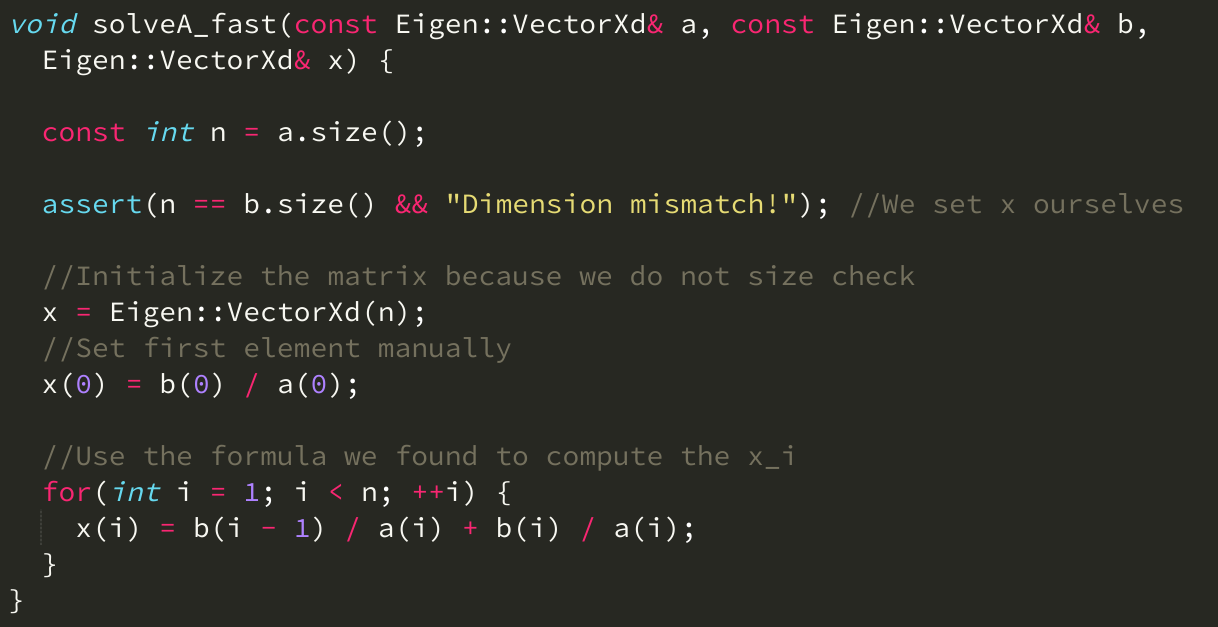
\includegraphics[width=1.0\linewidth]{2-12.e.png}
\end{figure}

\noindent In general given a triangular matrix ($\mathbf{A}$ is triangular) we can use \verb|triangularView| to tell Eigen that the system can be solved directly using backwards / forwards substitution. In this case this is more inefficient, however in general this approach could be used as well. Using \verb|triangularView| allows us to call \verb|solve()|, which is not possible on a regular matrix object.
\begin{figure}[!hbt]
    \centering
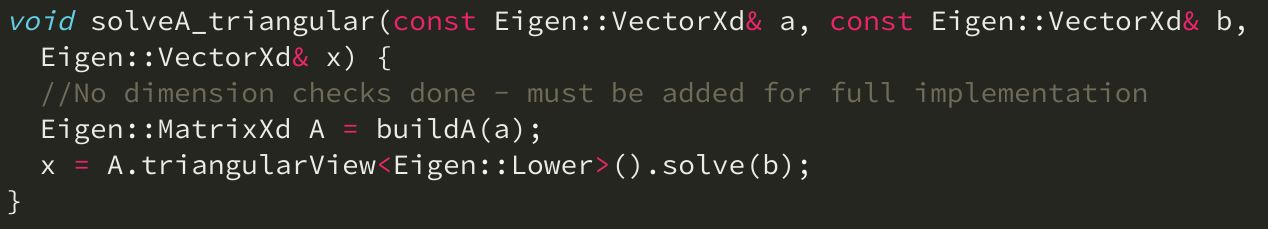
\includegraphics[width=0.9\linewidth]{2-12.etriag.png}
\end{figure}

\subsection*{2-12.f}
The following graph shows the timings of both method implemented (without the triangular one).

\begin{figure}[!hbt]
    \centering
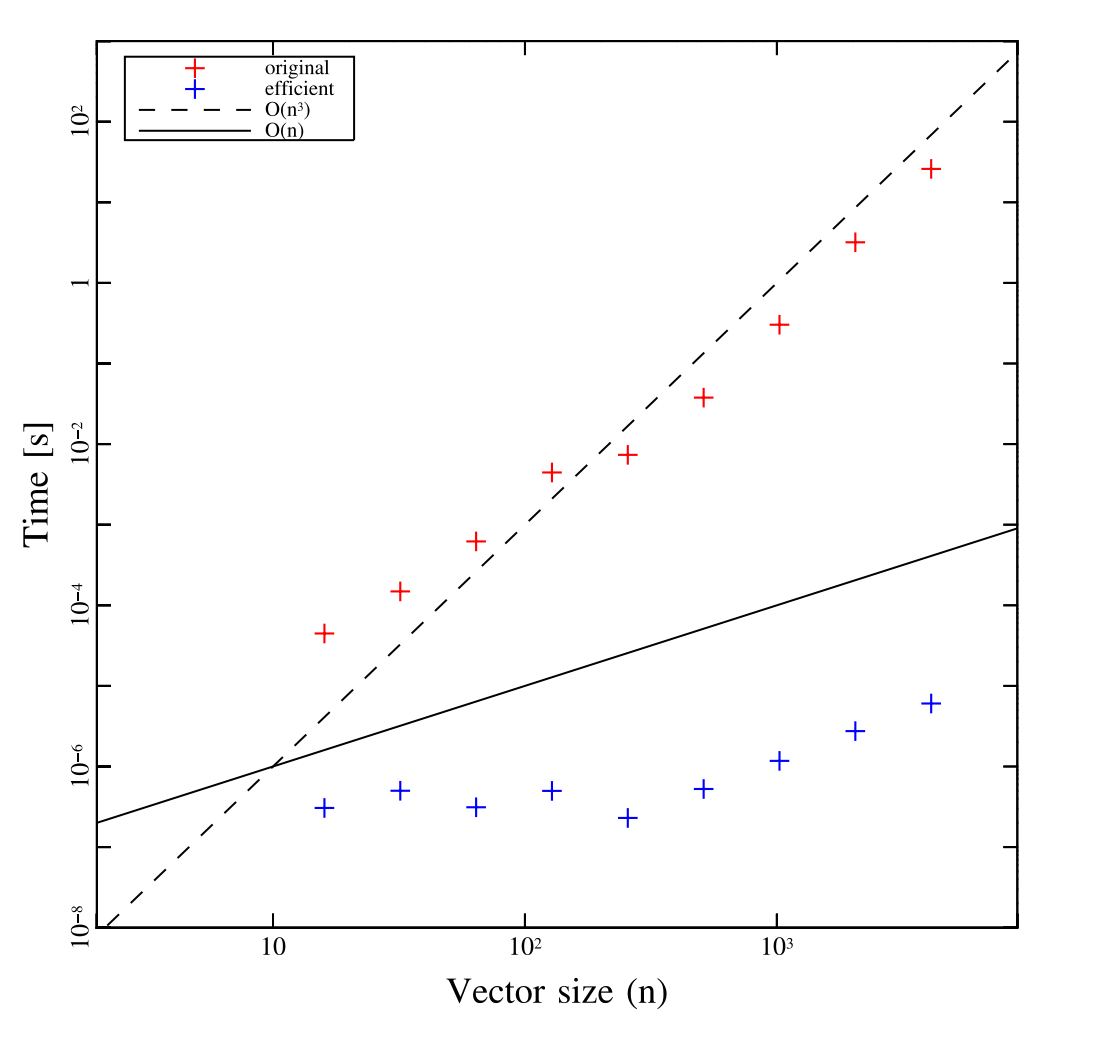
\includegraphics[width=0.9\linewidth]{2-12Timings.png}
\end{figure}

\end{document}
